\documentclass[UTF8]{ctexart}
\usepackage{graphicx}
\usepackage{amsmath}
\usepackage{geometry}
\usepackage{fancyhdr}
\usepackage{setspace}
\onehalfspacing
\addtolength{\parskip}{.4em}

% \geometry{papersize={20cm,40cm}}
% \geometry{left=1cm,right=2cm,top=3cm,bottom=4cm}

\title{你好,world!}
\author{Shang}
\date{\today}

\pagestyle{fancy}
\lhead{Shang}
\chead{\today}
\rhead{152xxxxxxxx}
\lfoot{}
\cfoot{\thepage}
\rfoot{}
\renewcommand{\headrulewidth}{0.4pt}
\renewcommand{\headwidth}{\textwidth}
\renewcommand{\footrulewidth}{0pt}

% 这里是导言区
\begin{document}
\maketitle
\tableofcontents
\section{你好中国}
中国

在East Asia.
\subsection{Hello Beijing}
北京是Capital of China.
\subsubsection{Hello Dongcheng District}
\paragraph{Tian'anmen Square}
is in the center of Beijing
\subparagraph{Chairman Mao}
is in the center of 天安门广场。
\subsection{Hello 山东}
\paragraph{山东大学} is one of the best university in 山东。

Hello, world!

Einstein 's $E=mc^2$.

\[ E=mc^ 2. \]
\begin{equation}
    E=mc^2.
\end{equation}

\begin{equation}
    z=r\cdot e^{2\pi i}.
\end{equation}

$\sqrt{x}$, $\dfrac{1}{2}$, $\tfrac{3}{4}$, $\frac{4}{5}$. 分式的尝试

\[ \sqrt{x}, \]
\[ \frac{1}{2}. \]

$ \sum_{i=1}^n i\quad \prod_{i=1}^n $
$ \sum\limits _{i=1}^n i\quad \prod\limits _{i=1}^n $
\[ \lim_{x\to0}x^2 \quad \int_a^b x^2 dx \]
\[ \lim\nolimits _{x\to0}x^2\quad \int\nolimits_a^b x^2 dx \]

\[ \iint\quad \iiint\quad \iiiint\quad \idotsint \]

\[ x_1,x_2,\dots ,x_n\quad 1,2,\cdots ,n\quad
\vdots\quad \ddots \]

\[ \Biggl(\biggl(\Bigl(\bigl((x)\bigr)\Bigr)\biggr)\Biggr) \]
\[ \Biggl[\biggl[\Bigl[\bigl[[x]\bigr]\Bigr]\biggr]\Biggr] \]
\[ \Biggl \{\biggl \{\Bigl \{\bigl \{\{x\}\bigr \}\Bigr \}\biggr \}\Biggr\} \]
\[ \Biggl\langle\biggl\langle\Bigl\langle\bigl\langle\langle x
\rangle\bigr\rangle\Bigr\rangle\biggr\rangle\Biggr\rangle \]
\[ \Biggl\lvert\biggl\lvert\Bigl\lvert\bigl\lvert\lvert x
\rvert\bigr\rvert\Bigr\rvert\biggr\rvert\Biggr\rvert \]
\[ \Biggl\lVert\biggl\lVert\Bigl\lVert\bigl\lVert\lVert x
\rVert\bigr\rVert\Bigr\rVert\biggr\rVert\Biggr\rVert \]

\[ \begin{pmatrix} a&b\\c&d \end{pmatrix} \quad
\begin{bmatrix} a&b\\c&d \end{bmatrix} \quad
\begin{Bmatrix} a&b\\c&d \end{Bmatrix} \quad
\begin{vmatrix} a&b\\c&d \end{vmatrix} \quad
\begin{Vmatrix} a&b\\c&d \end{Vmatrix} \]

Marry has a little matrix $ ( \begin{smallmatrix} a&b\\c&d \end{smallmatrix} ) $.

\begin{multline}
    x = a+b+c+{} \\
    d+e+f+g
\end{multline}

\begin{multline*}
    x = a+b+c+{} \\
    d+e+f+g
\end{multline*}

\[\begin{aligned}
    x ={}& a+b+c+{} \\
    &d+e+f+g
\end{aligned}\]

\begin{gather}
    a = b+c+d \\
    x = y+z
\end{gather}
\begin{align}
    a &= b+c+d \\
    x &= y+z
\end{align}

\[ y= \begin{cases}
    -x,\quad x\leq 0 \\
    x,\quad x>0
    \end{cases} \]

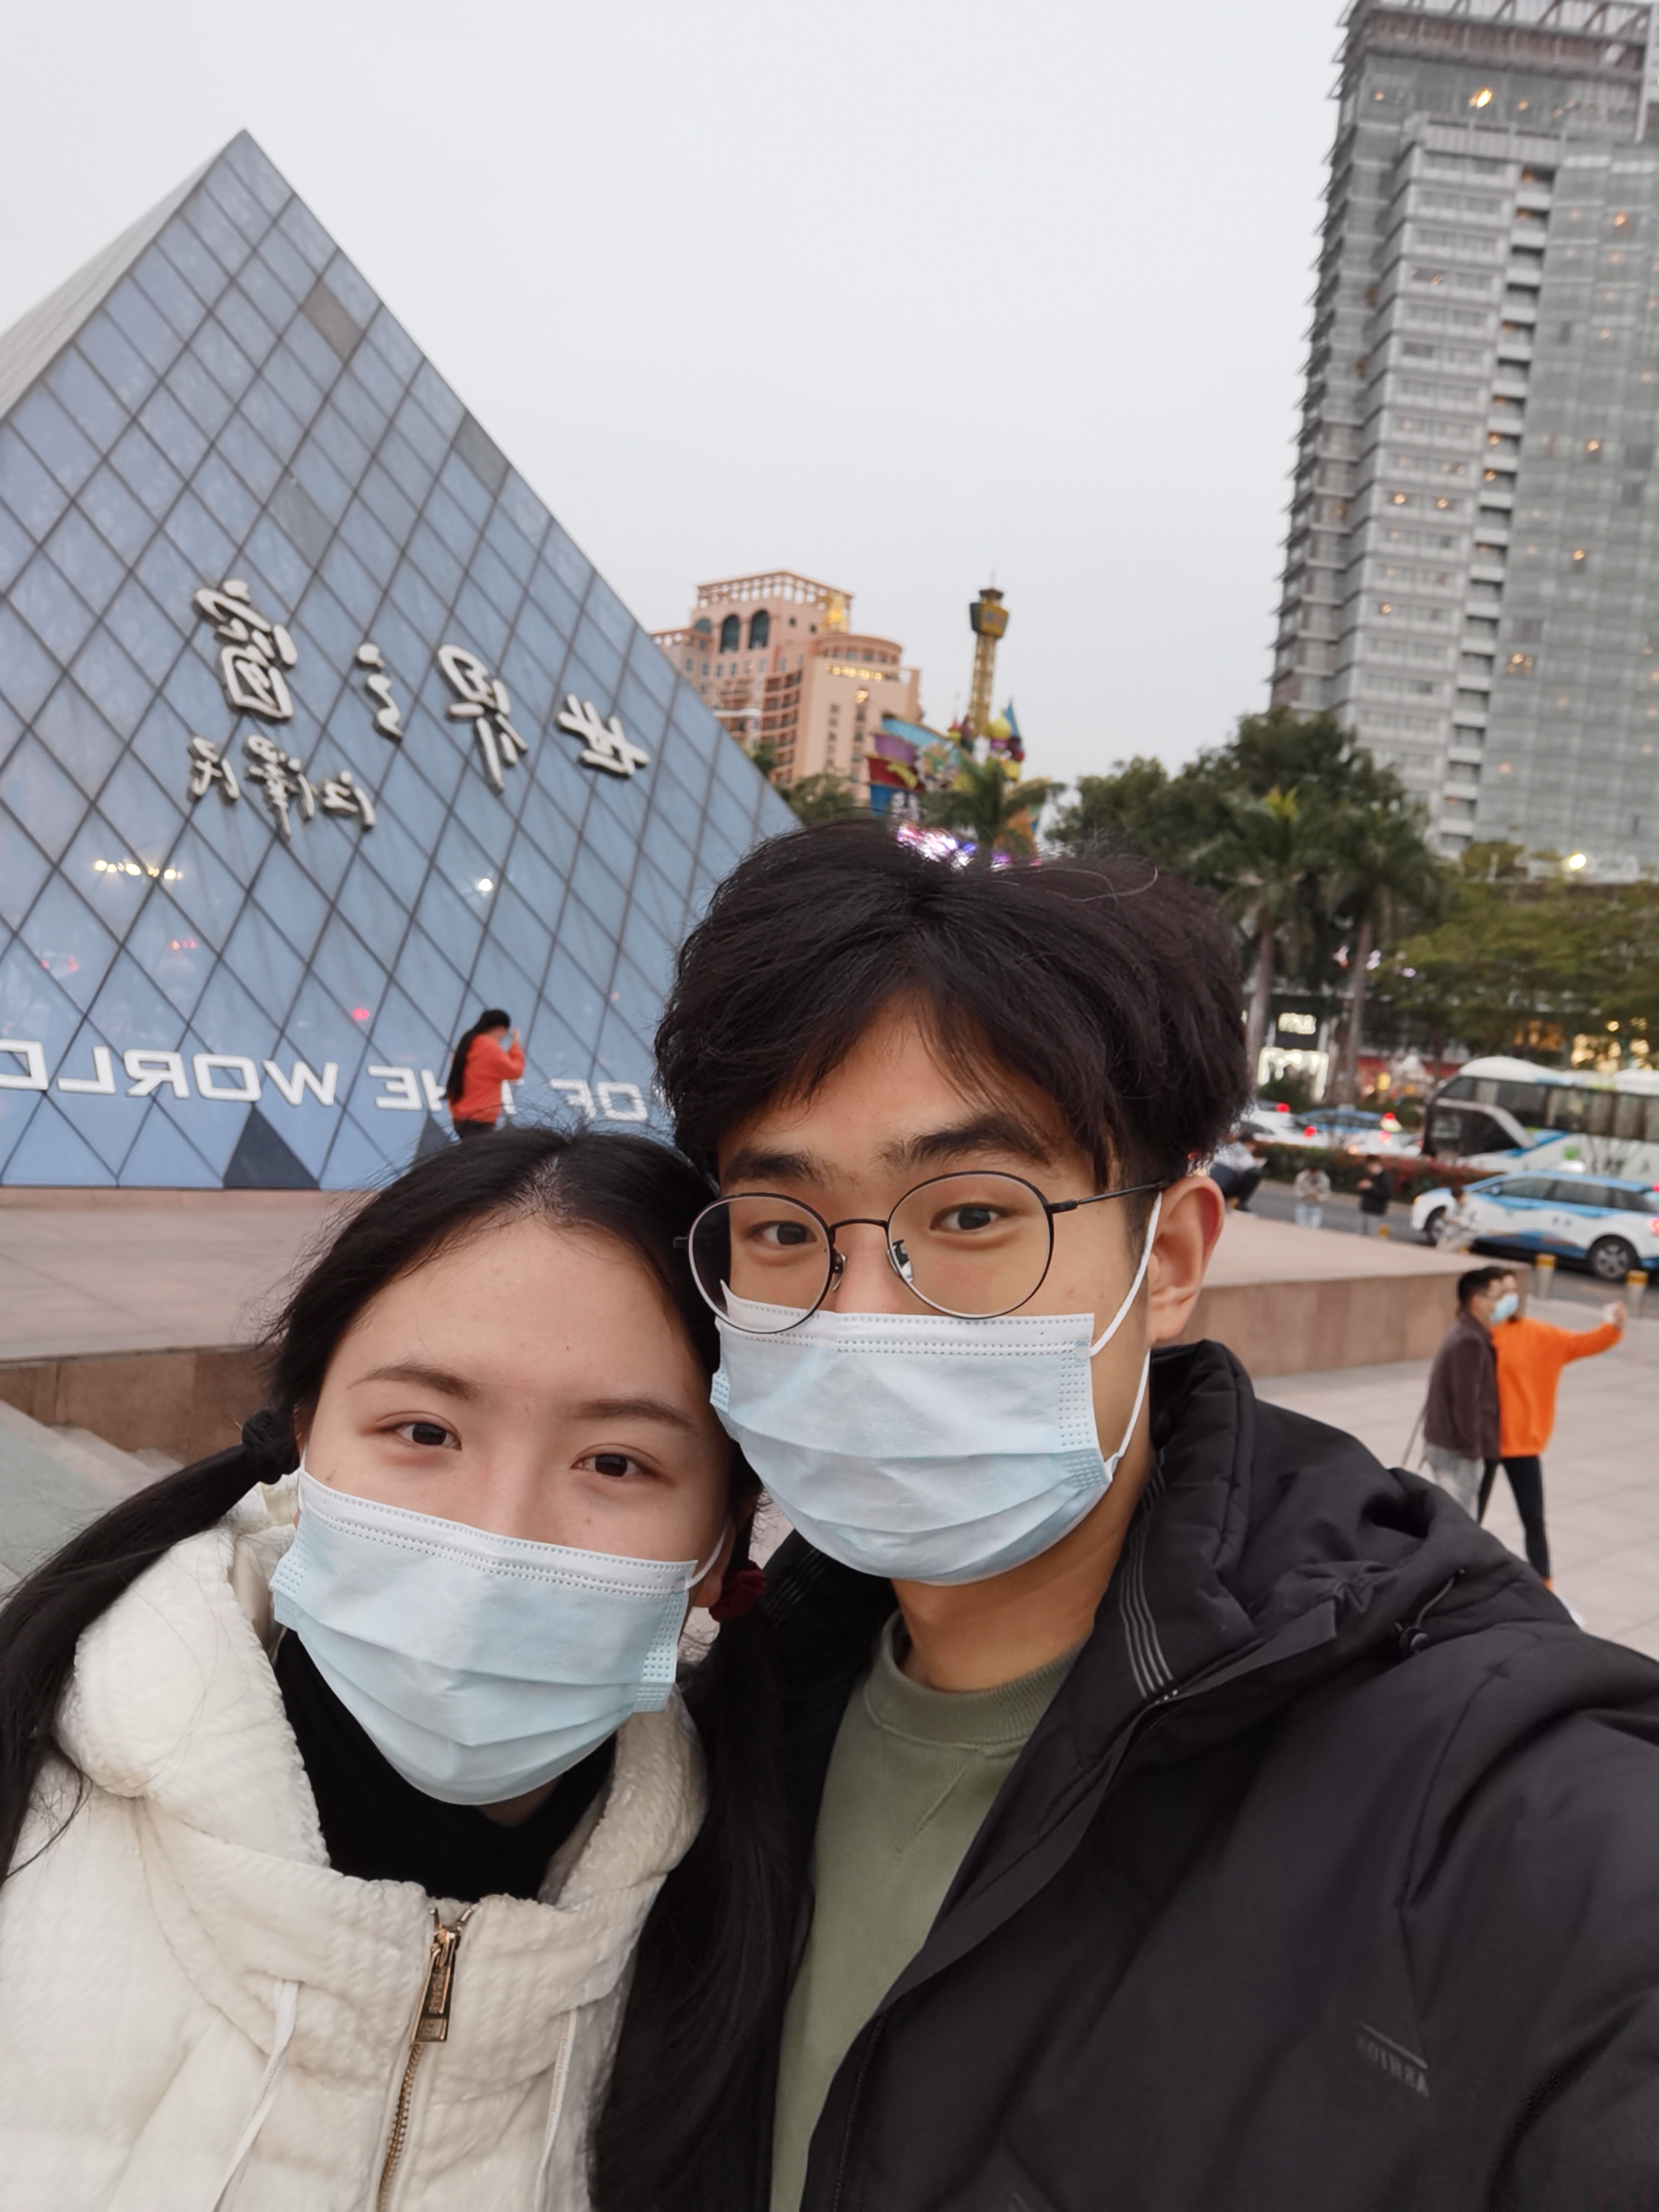
\includegraphics[width=.8\textwidth]{img/a.jpg}



\begin{tabular}{|l|c|r|}
    \hline
   操作系统& 发行版& 编辑器\\
    \hline
   Windows & MikTeX & TexMakerX \\
    \hline
   Unix/Linux & teTeX & Kile \\
    \hline
   Mac OS & MacTeX & TeXShop \\
    \hline
   通用& TeX Live & TeXworks \\
    \hline
\end{tabular}

\begin{figure}[htbp]
\centering
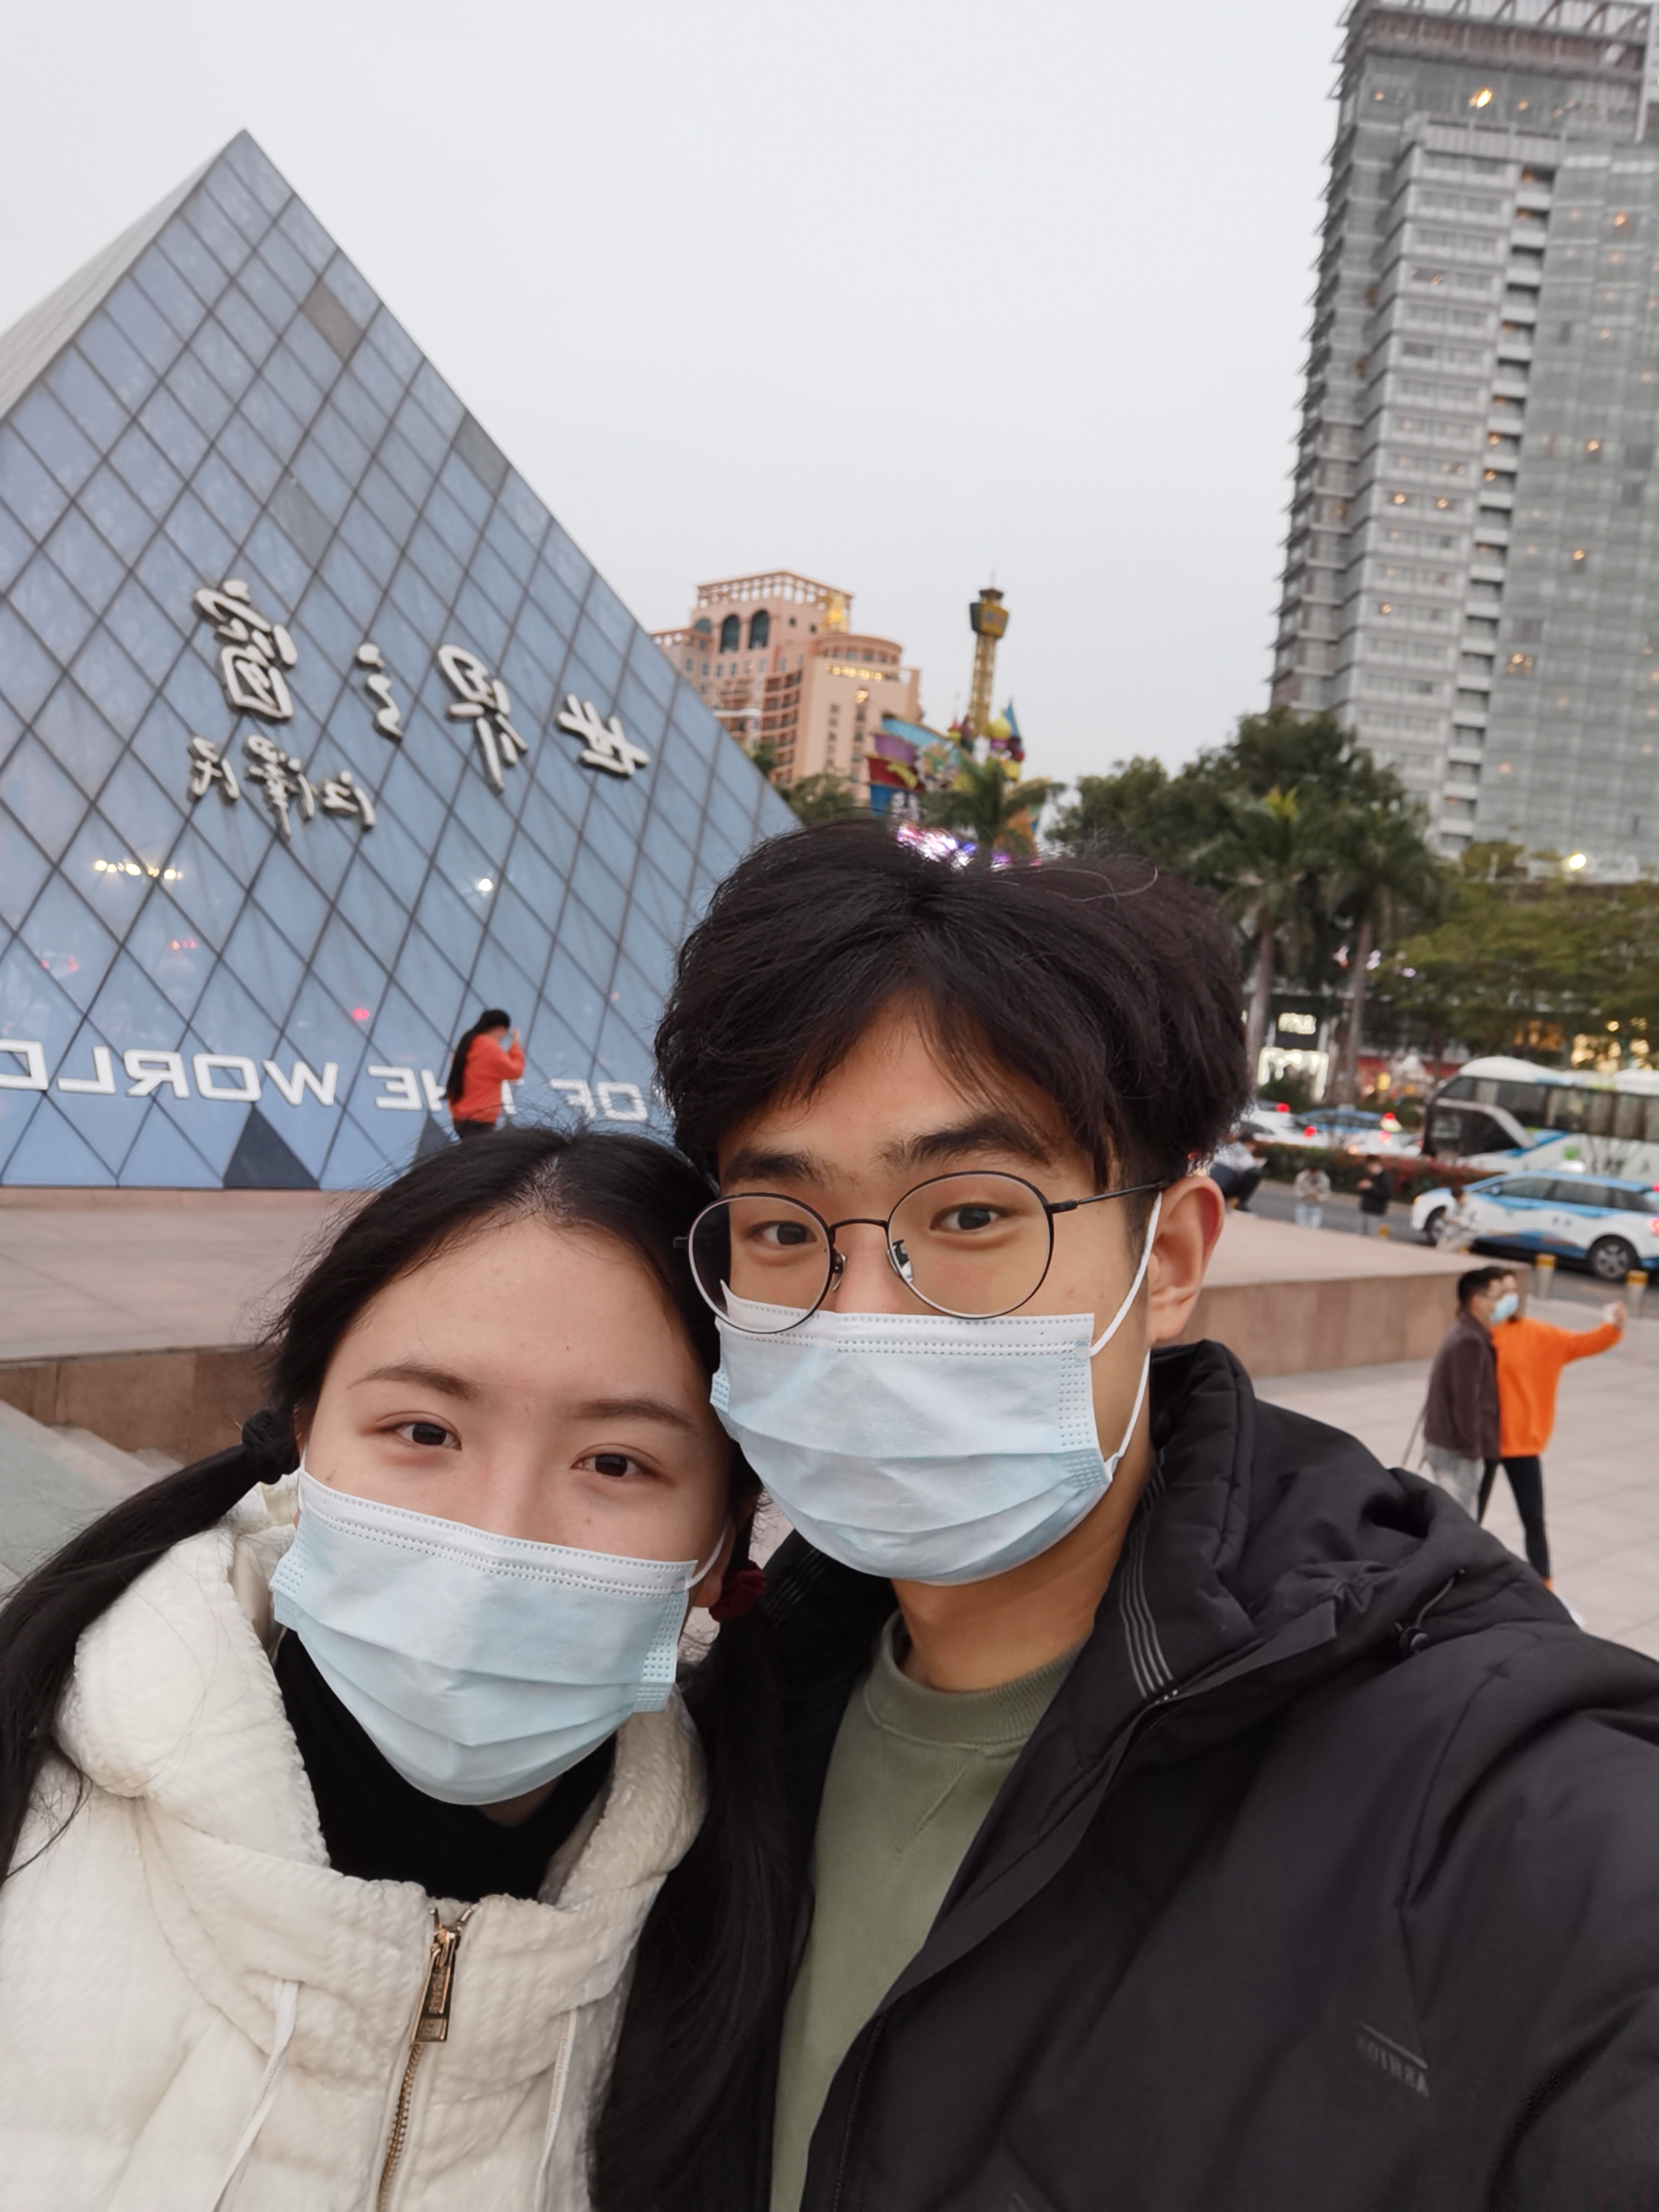
\includegraphics[width=.8\textwidth]{img/a.jpg}
\caption{有图有真相}
\label{fig:myphoto}
\end{figure}

\end{document}